\chapter{Introduction}


\begin{figure}
   \centering
   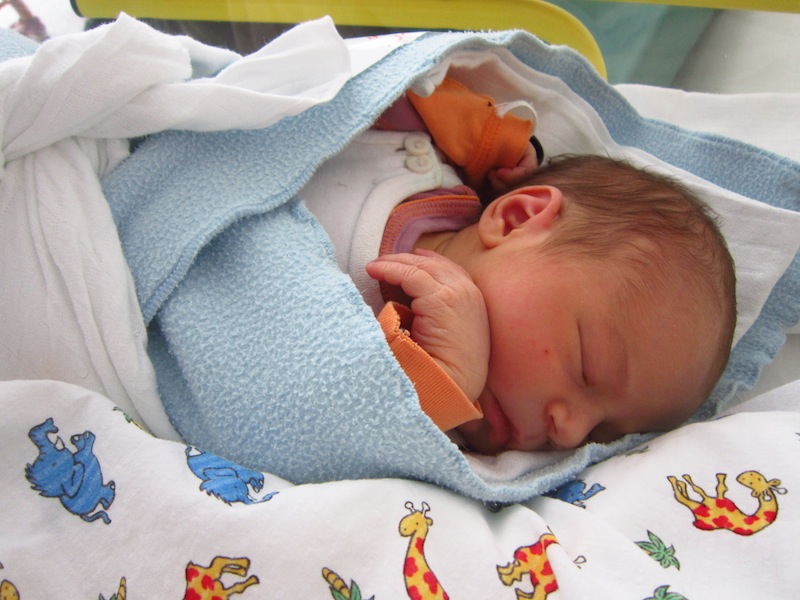
\includegraphics{example.jpg} % requires the graphicx package
   \caption{example caption}
   \label{fig:example}
\end{figure}

   
Co to je rendering
Zobrazovaci rovnice distribuce energie v prostoru. 

Co to je raytracing
paprsek protina geometrii v zakladu 

Jsou stale poupularnejsi progresivni metody renderingu, kdy se obraz pred stale vylepsuje, takze muzem videt nahled velice rychle.


ray tracing se stava poupularnejsi a popularnejsi, mene narocny na nastavovani a fizikalne korektni. Navic sceny jsou slozitejsi a slozitejsi divaci narocnejsi. 

Co to jsou volumetricke efekty a opticky aktivni prostredi

Avsak volumetricke efekty se stale dost casto rasterizujou.

Jak je to náročný a že se stále dost používají aproximační metody (rasterizace, deep shadow maps ) a nemodelují se náročné věci jako radiative transport surface to media volumetric caustics atd. Ani nástroje používané v produkci přímo nepodporuje a nebo jen v podobě náročných fotonových map, je to pomalé , takže artisti nemůžou odladit vse co chteji malo iteraci.



\section{Podkapitola}
